\begin{figure}[h]
	\centering
	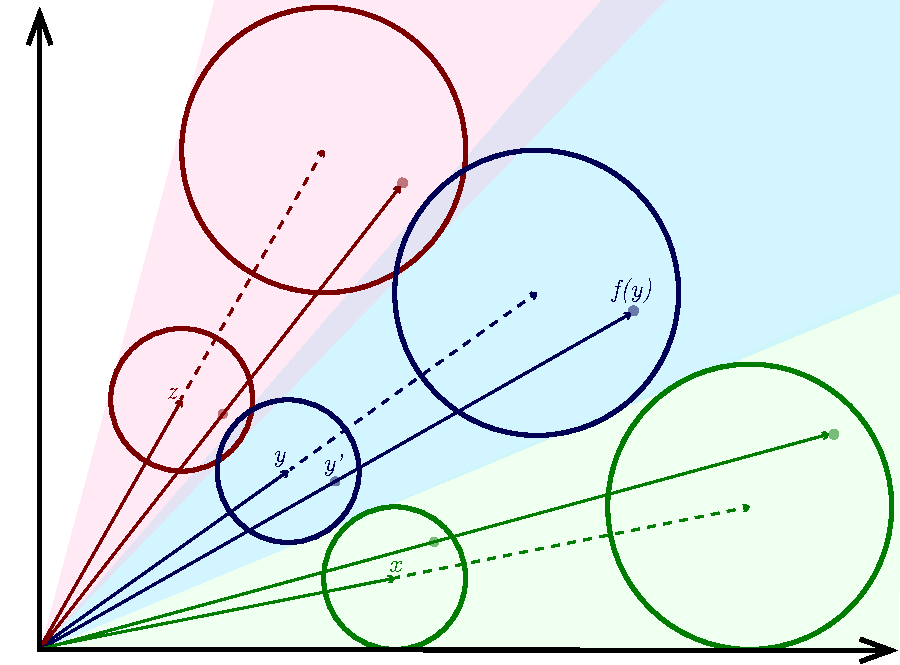
\includegraphics[width=1.0\textwidth]{dcpe}
	\caption[Schematic description of \acrshort{dcpe}]{
		Schematic description of encryption process of \acrshort{dcpe}, drawn to scale.
		In this diagram, there are two dimensions ($d = 2$), $\beta$ is 2 units, and $s$ is a factor of 2.
		The encrypted point is uniformly sampled inside a $\beta$-ball, then scaled $s$ times.
		If two points are too close, their circles intersect, and their encryptions can be sampled in way that breaks distance comparison.
		Intuitively, larger $\beta$ implies greater ciphertext space for a point and greater security.
	}\label{figure:dcpe}
\end{figure}
